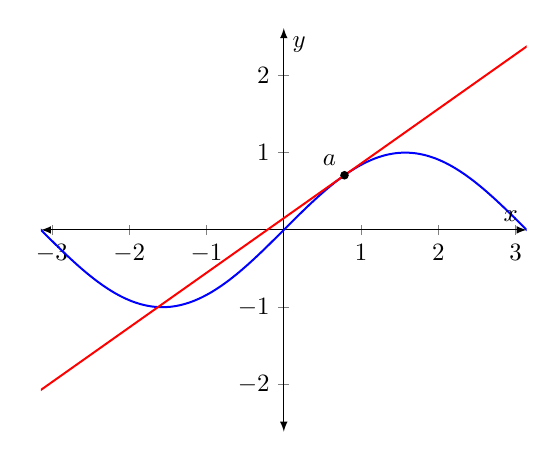
\begin{tikzpicture}[scale=0.90]
	\begin{axis}[
			% grid=both,
			xmin=-pi,
			xmax=pi,
			ymin=-1.6,
			ymax=1.6,
			axis lines=middle,
			xlabel = $x$,
			ylabel = $y$,
			axis line style={latex-latex},
      axis equal,
		]

		\addplot[
			samples=200,
			domain=-4*pi:4*pi,
			color=blue,
			thick,
			smooth,
		]
		{sin(deg(x))};

		\addplot[
			domain=-5:5,
			color=red,
      thick,
		]{( (sqrt(2) / 2) * (x - (pi/4)) ) +  (sqrt(2) / 2)};

		\addplot+[
			mark options={black},
      mark size=1.5pt,
		] coordinates {(0.785398,0.707106)} node [black, left=6pt, above=0.5pt] {$a$};
	\end{axis}
\end{tikzpicture}

